\chapter{Intrinsically Disordered Proteins}
\label{ch:disorder}

For decades, the central dogma of structural biology was ``structure determines function.''
Anfinsen's thermodynamic hypothesis, the lock-and-key model, and the success of X-ray
crystallography all reinforced a single idea: a protein's biological activity depends on a
well-defined three-dimensional fold.  But by the late 1990s, Wright and
Dyson~\cite{wright1999}, and independently Dunker and colleagues~\cite{dunker2001},
accumulated evidence that many functional proteins lack stable tertiary structure under
physiological conditions.  The p53 transactivation domain, which binds MDM2 and activates
transcription, is fully disordered in isolation~\cite{kussie1996}.  It folds only upon
binding its partner.  The crystallographers had not failed to solve these structures.  The
structures did not exist.

This chapter treats proteins that break the structure-function rule.  We begin with the
physics of disordered polypeptide chains, treating them as statistical ensembles rather than
single conformations.  We then develop computational methods for predicting disorder from
sequence, discuss how disordered regions contribute to biological function, and close with
the connection between low-complexity disordered domains and liquid-liquid phase separation
in cells.

%% ======================================================================
\section{Biophysics of Disorder}
\label{sec:disorder-biophysics}
%% ======================================================================

A folded protein occupies a narrow basin in conformational space.  An intrinsically
disordered protein (IDP) does not.  Under native conditions, an IDP samples a broad
distribution of conformations, and no single structure represents the molecule
adequately.\sidenote{The term ``intrinsically disordered'' was popularized by Dunker
et~al.~\cite{dunker2001}.  Wright and Dyson~\cite{wright1999} used ``intrinsically
unstructured.''  Both terms refer to the same phenomenon: functional proteins that lack a
fixed tertiary fold under physiological conditions.}  The correct description is an
ensemble: a probability distribution over the space of backbone dihedral angles, weighted by
the Boltzmann factor $e^{-E/k_BT}$.

\begin{figure*}
  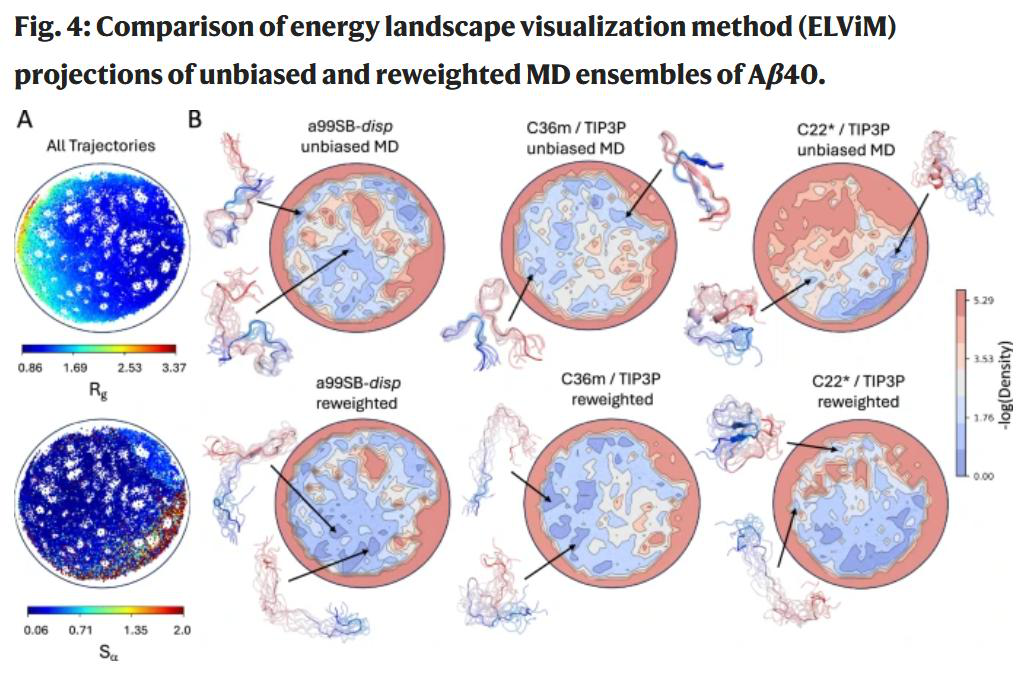
\includegraphics[width=\linewidth]{figures/ch11_idp_ensemble.png}
  \caption{Conformational ensemble of the A$\beta$40 intrinsically disordered peptide.}
  \label{fig:idp-ensemble}
\end{figure*}

Experimentally, this ensemble manifests in specific ways.  In NMR spectroscopy, disordered
regions show narrow chemical shift dispersion, because the rapid interconversion between
conformers averages the local magnetic environments.  In small-angle X-ray scattering
(SAXS), IDPs produce scattering profiles consistent with extended, flexible chains rather
than compact globules.  Circular dichroism spectra of IDPs typically show a strong negative
band near 200~nm and weak signal at 222~nm, indicating the absence of stable
$\alpha$-helical or $\beta$-sheet content.

\newthought{The simplest physical model} for a disordered chain is the random coil.
Consider a polymer of $N$ bonds, each of length $l$, with the direction of each bond chosen
independently.  The mean-square end-to-end distance of a freely jointed chain is
%
\begin{equation}
  \langle R^2 \rangle_{\text{free}} = N \, l^2.
  \label{eq:freely-jointed}
\end{equation}

Real polypeptide chains are not freely jointed.  Bond angles are constrained, and rotations
around backbone bonds are correlated over short distances.  Flory accounted for these local
stiffness effects with the characteristic ratio
$C_N$:\sidenote{Paul Flory developed the statistical mechanics of polymer chains in the
1950s and 1960s.  His 1969 monograph \textit{Statistical Mechanics of Chain
Molecules}~\cite{flory1969} remains the standard reference.  Flory won the Nobel Prize in
Chemistry in 1974.}
%
\begin{equation}
  \langle R^2 \rangle = C_N \cdot N \cdot l^2,
  \label{eq:flory-random-coil}
\end{equation}
%
\noindent where $C_N$ captures the deviation from ideal random-walk statistics due to fixed
bond angles and short-range steric effects.  For polypeptides, $C_N$ typically ranges from 8
to 12, depending on the amino acid composition.  A high proline content, for instance,
stiffens the backbone and increases $C_N$.  As $N \to \infty$, $C_N$ converges to the
characteristic ratio $C_\infty$.

\newthought{Beyond local stiffness,} the long-range behavior of polymer chains depends on
the balance between chain-chain and chain-solvent interactions.  This balance is captured by
the scaling exponent $\nu$ in the relation
%
\begin{equation}
  R_g \sim N^{\nu},
  \label{eq:scaling-law}
\end{equation}
%
\noindent where $R_g$ is the radius of gyration.  Three regimes matter.  In a good solvent,
where monomer-solvent contacts are favored over monomer-monomer contacts, excluded volume
effects swell the chain.  Flory's mean-field argument gives $\nu = 3/5$; the more precise
renormalization group result is $\nu = 0.588$.\sidenote{The Flory exponent $\nu = 3/(d+2)$
gives $\nu = 3/5 = 0.6$ in three dimensions.  The exact value from renormalization group
theory is $\nu \approx 0.588$~\cite{degennes1979}.  The difference is small but measurable
in careful SAXS experiments on long IDPs.}  In a theta solvent, where attractive and
repulsive interactions exactly cancel, the chain behaves as an ideal random walk with $\nu =
1/2$.  In a poor solvent, where monomer-monomer contacts are preferred, the chain collapses
into a compact globule with $\nu = 1/3$.

For IDPs in aqueous solution, the effective solvent quality depends on the amino acid
sequence.  Highly charged, low-hydrophobicity sequences behave as expanded chains with $\nu$
near 0.588.  Sequences with more hydrophobic residues adopt more compact ensembles, with
$\nu$ approaching 1/3.  Folded proteins represent the extreme of this spectrum: they are
effectively in a poor solvent for their own backbone, collapsed into a state where $\nu
\approx 1/3$ and the packing density approaches that of organic crystals.

\newthought{What determines whether} a protein is ordered or disordered?  Two sequence
properties are strong predictors: mean hydrophobicity and mean net
charge~\cite{uversky2000}.  Ordered proteins tend to have higher hydrophobicity (which
stabilizes the hydrophobic core) and lower net charge (which reduces electrostatic repulsion
within the folded state).  Disordered proteins invert this pattern: their sequences are
enriched in charged and polar residues (Glu, Asp, Lys, Arg, Gln, Ser, Pro) and depleted in
hydrophobic residues (Ile, Leu, Val, Trp, Phe, Tyr).

Uversky and colleagues formalized this observation with the charge-hydropathy
plot~\cite{uversky2000}.  On this plot, the $x$-axis is the mean absolute net charge per
residue $\langle |q| \rangle / N$, and the $y$-axis is the mean Kyte-Doolittle
hydrophobicity $\langle H \rangle$.  A linear boundary separates ordered and disordered
proteins with reasonable accuracy:
%
\begin{equation}
  \langle H \rangle_{\text{boundary}}
    = \frac{\langle |q| \rangle / N + 1.151}{2.785}.
  \label{eq:uversky-boundary}
\end{equation}
%
\noindent Proteins above this line (high hydrophobicity, low charge) tend to fold.  Proteins
below it (low hydrophobicity, high charge) tend to be
disordered.\sidenote{The Uversky plot is a useful heuristic, but it captures only two of
many relevant sequence features.  Proline content, for example, disrupts secondary
structure.  Low-complexity regions (polyQ, polyN) are often disordered despite moderate
hydrophobicity.  More recent predictors incorporate dozens of features.}

A third sequence property associated with disorder is low complexity.  Many IDPs contain
long stretches of repetitive or compositionally biased sequence: polyglutamine tracts,
serine/arginine-rich regions, glycine-rich loops.  These sequences lack the information
content needed to specify a unique fold.  We return to low-complexity domains in the context
of phase separation later in this chapter.


%% ======================================================================
\section{Disorder Prediction}
\label{sec:disorder-prediction}
%% ======================================================================

Given the difficulty of characterizing disordered proteins experimentally (they resist
crystallization, and NMR ensemble methods are labor-intensive), computational prediction
from amino acid sequence has become the primary tool for identifying disordered regions at
scale.

\newthought{The IUPred algorithm,} developed by Doszt\'anyi and
colleagues~\cite{dosztanyi2005,meszaros2018}, takes a physicochemical approach.  The
central idea is that ordered regions form enough stabilizing pairwise contacts to compensate
for the conformational entropy lost upon folding, while disordered regions cannot.  IUPred
estimates the pairwise interaction energy for each residue based on a statistical potential
derived from globular protein structures.  For residue $i$, the estimated energy is
%
\begin{equation}
  \Delta G_i = \sum_{j} f(r_{ij}) \cdot e_{ij},
  \label{eq:iupred-energy}
\end{equation}
%
\noindent where the sum runs over residues $j$ within a sequence window, $e_{ij}$ is a
statistical potential that depends on the amino acid types at positions $i$ and $j$, and
$f(r_{ij})$ is a weighting function that depends on the sequence separation
$|i-j|$.\sidenote{IUPred does not use three-dimensional coordinates.  The term $r_{ij}$
here refers to sequence distance, not spatial distance.  The statistical potential was
parameterized from contact maps of known globular structures, then applied to predict
contacts for novel sequences.}  Residues that are predicted to form many favorable contacts
(low $\Delta G_i$) are classified as ordered.  Residues with few predicted favorable
contacts (high $\Delta G_i$) are classified as disordered.

The updated version, IUPred2A~\cite{meszaros2018}, introduced context-dependent
predictions.  A protein's disorder state may change depending on its redox environment
(cysteine-rich regions can form disulfide bonds under oxidizing conditions, stabilizing
structure) or whether it is bound to a partner.  IUPred2A models these effects by adjusting
the energy calculation to account for additional stabilizing interactions present under
specific cellular conditions.

\newthought{An alternative class of predictors} exploits compositional bias directly.  These
methods train classifiers on the amino acid composition of known disordered and ordered
regions.  The simplest version computes a per-residue disorder propensity based on the
frequency of each amino acid type in experimentally verified disordered regions versus
ordered regions from the Protein Data Bank.  Residues in regions enriched in
disorder-promoting amino acids (Ala, Arg, Gly, Gln, Ser, Glu, Lys, Pro) score high, while
residues in regions enriched in order-promoting amino acids (Trp, Cys, Phe, Ile, Tyr, Val,
Leu) score low.  These methods are fast and interpretable, though they miss
context-dependent effects that arise from the specific sequence neighborhood.

\newthought{Because individual predictors} have complementary strengths, meta-predictors
combine their outputs.  MobiDB-lite~\cite{necci2021} runs multiple disorder prediction
algorithms in parallel and assigns a consensus disorder annotation.  A residue is labeled
disordered only if a majority of the constituent methods agree.  This consensus approach
reduces the false positive rate at the cost of some sensitivity, producing annotations that
are more conservative but more reliable than any single method.

\newthought{A surprising recent development} came from AlphaFold~\cite{jumper2021}.  The
predicted Local Distance Difference Test (pLDDT) score, which AlphaFold produces as a
per-residue confidence estimate, turns out to be a strong disorder predictor.  Regions where
AlphaFold reports low confidence (pLDDT $< 50$) correspond closely to experimentally
validated disordered regions~\cite{tunyasuvunakool2021}.  This makes intuitive sense:
AlphaFold was trained on protein structures from the PDB, so residues that have no
well-defined structure in nature should produce low-confidence predictions.  The entire
AlphaFold Protein Structure Database can thus be mined for disorder annotations by
thresholding pLDDT, providing proteome-wide disorder maps at no additional computational
cost beyond the structure predictions themselves.\sidenote{There is a subtlety here.  Low
pLDDT could indicate genuine intrinsic disorder, but it could also flag regions where
AlphaFold simply lacks sufficient evolutionary information (poor MSA quality).  In practice,
for well-covered sequences, the correlation between low pLDDT and experimental disorder is
strong.}

\begin{marginfigure}
  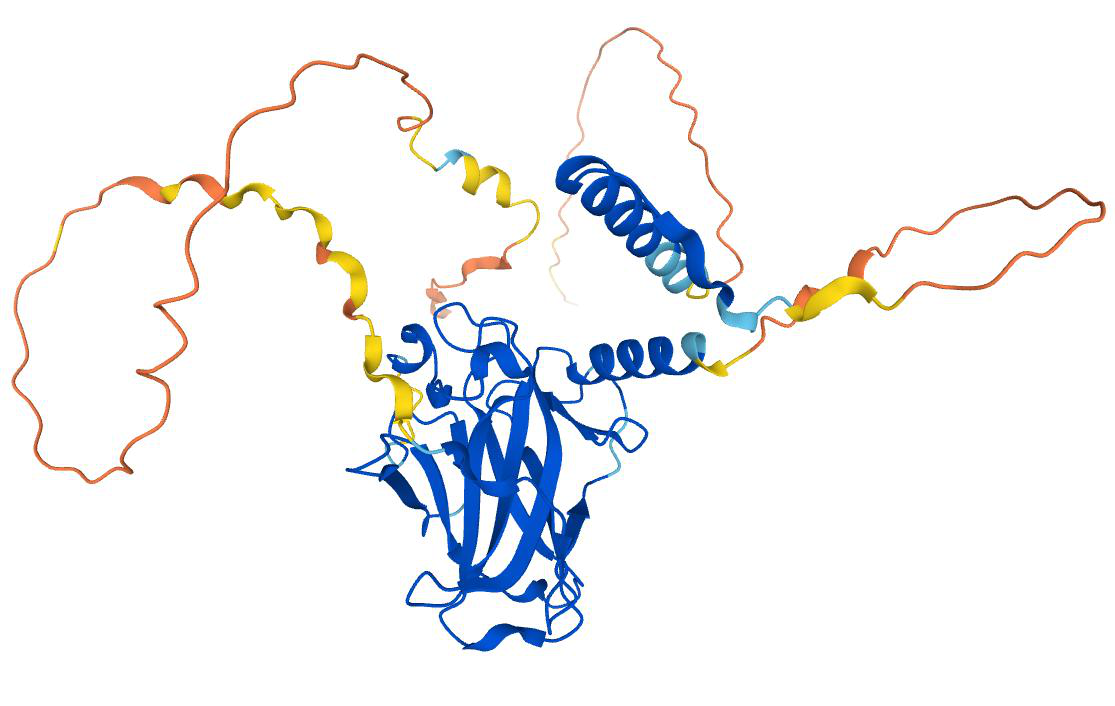
\includegraphics[width=\linewidth]{figures/ch11_plddt_disorder.png}
  \caption{AlphaFold pLDDT coloring reveals disordered regions.}
  \label{fig:plddt-disorder}
\end{marginfigure}


%% ======================================================================
\section{Functional Disorder}
\label{sec:functional-disorder}
%% ======================================================================

The existence of disordered proteins would be unremarkable if they were merely non-functional
linkers between globular domains.  They are not.  Disordered regions are central to
signaling, transcription, and regulation across all domains of life, and their prevalence
increases with organism complexity.\sidenote{In \textit{E.~coli}, roughly 4\% of proteins
contain long disordered regions ($>30$ consecutive disordered residues).  In humans, the
fraction exceeds 30\%~\cite{oldfield2014}.  The expansion of disorder correlates with the
expansion of regulatory complexity in eukaryotes.}  The question is how a region without a
fixed structure can perform specific biological functions.

\newthought{Molecular Recognition Features} (MoRFs) provide one answer.  A MoRF is a short
segment, typically 10--70 residues, within a longer disordered region that undergoes a
disorder-to-order transition upon binding a structured partner~\cite{oldfield2014}.  The p53
transactivation domain mentioned in the opening is a canonical MoRF: its 15-residue segment
(residues 18--26) forms an $\alpha$-helix only when bound to the hydrophobic cleft of
MDM2~\cite{kussie1996}.  In isolation, this segment samples a heterogeneous ensemble of
extended and partially helical conformations.

\begin{marginfigure}
  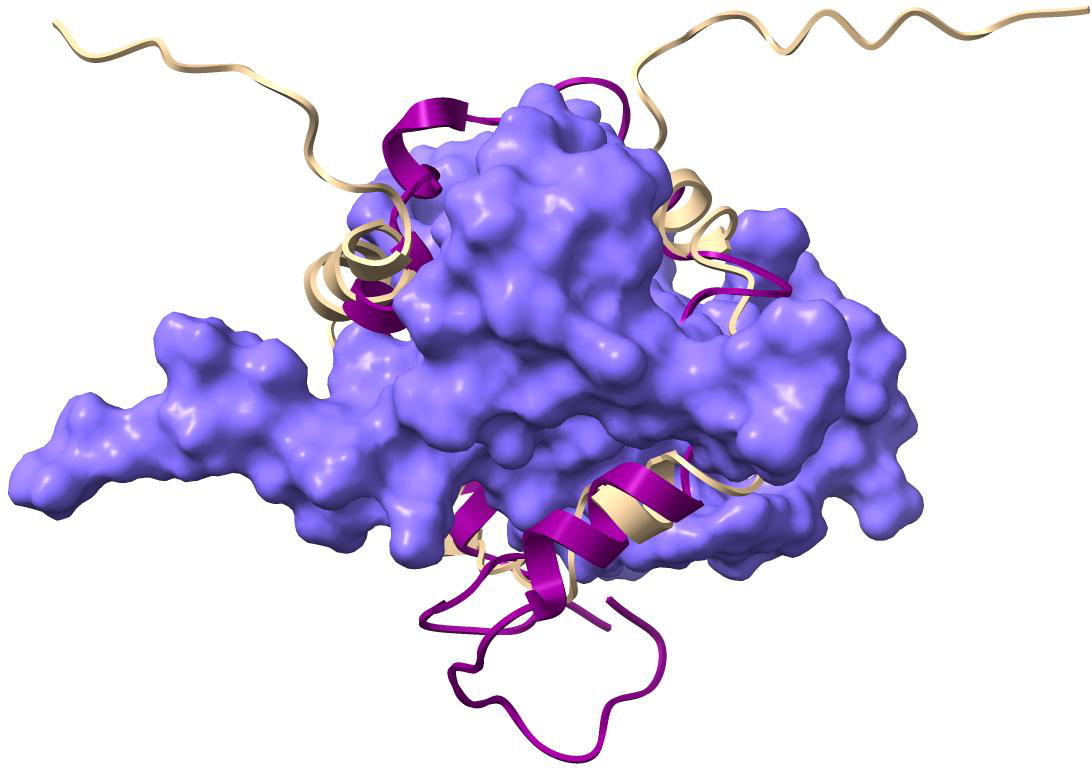
\includegraphics[width=\linewidth]{figures/ch11_coupled_folding.png}
  \caption{Coupled folding and binding of a disordered protein.}
  \label{fig:coupled-folding}
\end{marginfigure}

The thermodynamic cost of this coupled folding and binding reaction is real.  The MoRF must
pay an entropic penalty to adopt a single conformation, which reduces the net binding free
energy compared to a pre-folded peptide binding the same site.  Why, then, has evolution
preserved this apparently wasteful mechanism?  One advantage is specificity without excessive
affinity.  Signaling interactions often require binding that is tight enough to be specific
but weak enough to be rapidly reversible.  The entropic penalty of folding upon binding tunes
the $K_d$ into the micromolar range, appropriate for transient signaling interactions, even
when the enthalpic contacts at the interface are
extensive.\sidenote{This is sometimes called the ``entropic counterweight'' principle.  A
pre-folded helix binding MDM2 would have a $K_d$ in the nanomolar range or tighter, which
would make the interaction too stable for rapid signaling.}

\newthought{Short Linear Motifs} (SLiMs), also called Eukaryotic Linear Motifs (ELMs), are a
related but distinct class of functional elements in disordered
regions~\cite{vanderlee2014,davey2012}.  SLiMs are short peptide segments, typically 3--10
residues, defined by a consensus sequence pattern.  They mediate protein-protein
interactions, post-translational modifications, and subcellular targeting.  The PxIxIT motif
that binds calcineurin, the LXCXE motif that binds retinoblastoma protein, and the PY-NLS
motif recognized by importin-$\beta$ are well-characterized examples.

SLiMs are overwhelmingly located in disordered regions, and this is not coincidental.  A
SLiM must be accessible to its binding partner, and burial within a globular core would
prevent this.  Disorder provides the conformational flexibility needed for the motif to adopt
the correct geometry upon binding.  The compactness of the motif (often only 3--5
specificity-determining residues) means that it can evolve rapidly: a few point mutations in
a disordered tail can create or destroy a SLiM, rewiring a signaling pathway without
disrupting the protein's folded domains.

\newthought{The ``fly-casting'' mechanism,} proposed by Shoemaker, Portman, and
Wolynes~\cite{shoemaker2000}, offers a kinetic rationale for coupled folding and binding.
Consider a disordered protein searching for its binding partner by diffusion.  In its
extended, disordered state, the protein has a larger hydrodynamic radius than it would in a
compact, folded conformation.  This extended state increases the capture radius for the
initial encounter with the target.  Once contact is made, the disordered protein folds
around its partner, locking in the specific interactions.

The quantitative argument proceeds as follows.  The diffusion-limited association rate
$k_{\text{on}}$ for two spherical molecules scales with the sum of their radii:
%
\begin{equation}
  k_{\text{on}} \sim D \cdot (R_1 + R_2),
  \label{eq:fly-casting}
\end{equation}
%
\noindent where $D$ is the relative diffusion coefficient and $R_1$, $R_2$ are the effective
radii.  An extended disordered chain with $R_g \sim N^{0.588}$ presents a larger target than
a compact folded domain with $R_g \sim N^{1/3}$.  For a 100-residue segment, the ratio is
roughly $(100^{0.588}) / (100^{0.333}) \approx 15 / 4.6 \approx 3.2$, a threefold
enhancement in effective capture radius.  The tradeoff is that not all initial contacts are
productive: the disordered chain must find the correct binding mode through a combination of
sliding and local folding, which introduces a kinetic cost.  Whether fly-casting provides a
net kinetic advantage depends on the balance between these effects, and the evidence suggests
it does for many IDP-target interactions where the initial encounter is rate-limiting.

\newthought{Not all disorder disappears} upon binding.  Tompa and Fuxreiter introduced the
concept of ``fuzzy complexes'' to describe protein-protein interactions in which one or both
partners retain significant disorder in the bound state~\cite{tompa2005}.  In a fuzzy
complex, the disordered regions do not fold into a single conformation upon binding.
Instead, they remain dynamic, sampling multiple conformations while maintaining the
interaction.

The Sic1-Cdc4 interaction in yeast cell-cycle regulation is a well-studied example.  Sic1
contains multiple phosphorylation sites in a disordered region.  When phosphorylated, these
sites bind the WD40 domain of Cdc4, but Sic1 remains largely disordered in the complex.
The binding depends on the total number of phosphorylated residues rather than any single
phosphosite, suggesting a polyelectrostatic interaction where multiple weak, transient
contacts collectively stabilize the complex.  This ``ultrasensitive'' binding, requiring a
threshold number of phosphorylations before Sic1 is recognized by Cdc4, acts as a molecular
switch for cell-cycle progression.

\begin{figure}
  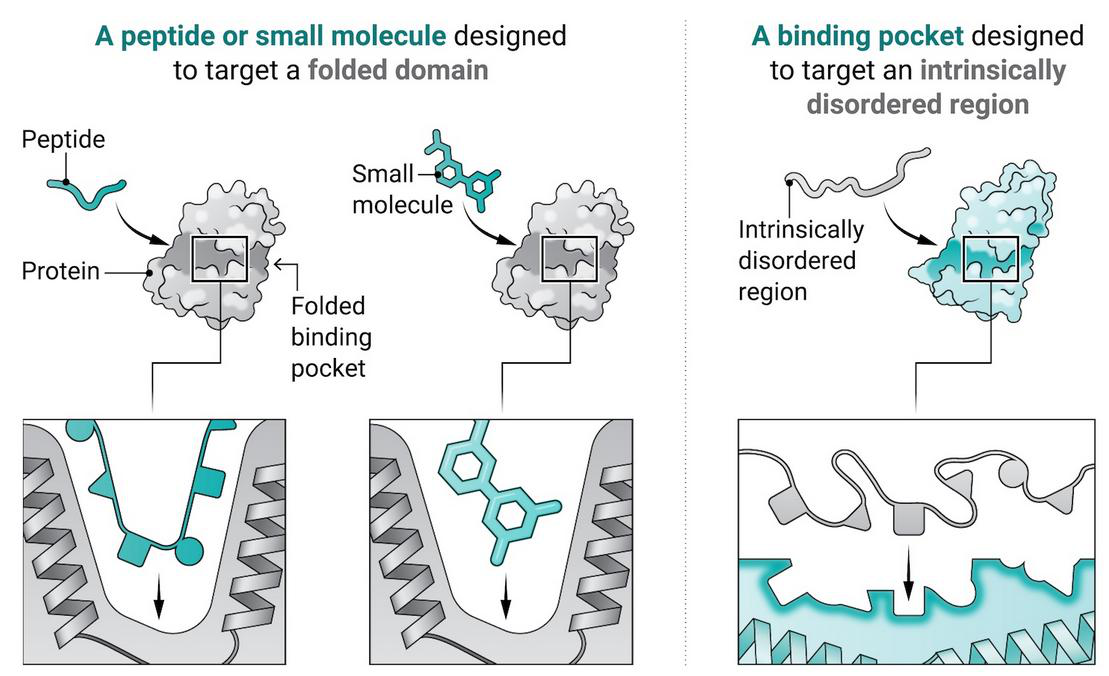
\includegraphics[width=\linewidth]{figures/ch11_targeting_idps.png}
  \caption{Strategies for targeting folded versus intrinsically disordered proteins.}
  \label{fig:targeting-idps}
\end{figure}


%% ======================================================================
\section{Phase Separation and Low-Complexity Domains}
\label{sec:phase-separation}
%% ======================================================================

In 2009, Brangwynne, Hyman, and J\"ulicher reported that P~granules in
\textit{C.~elegans} embryos behave as liquid droplets~\cite{brangwynne2009}.  These
membrane-less organelles fuse, drip, and dissolve in response to concentration changes,
exactly as expected for a liquid phase coexisting with the surrounding cytoplasm.  The
discovery that cells use liquid-liquid phase separation (LLPS) to organize their interiors
opened a new field at the intersection of polymer physics and cell
biology.\sidenote{Membrane-less organelles had been observed for over a century (the
nucleolus was described in the 1830s), but their physical nature was not understood until the
Brangwynne et~al.\ experiments.  The language of phase transitions gave biologists a
quantitative framework for thinking about these structures.}

\newthought{The thermodynamics of LLPS} follow from classical polymer solution theory.
Consider a solution of multivalent macromolecules.  At low concentrations, the molecules are
dispersed.  Above a threshold concentration $c_{\text{sat}}$ (the saturation concentration),
the solution separates into a dilute phase (at concentration $c_{\text{sat}}$) and a dense
phase (at concentration $c_{\text{dense}}$).  The driving force for phase separation is that
the free energy of the homogeneous solution exceeds that of the two-phase system: the
favorable interactions in the dense phase outweigh the entropy of mixing lost by
concentrating the molecules.

The Flory-Huggins free energy of mixing for a polymer solution is
%
\begin{equation}
  \frac{\Delta G_{\text{mix}}}{k_B T}
    = \frac{\phi}{N} \ln \phi
    + (1 - \phi) \ln(1 - \phi)
    + \chi \, \phi \, (1 - \phi),
  \label{eq:flory-huggins}
\end{equation}
%
\noindent where $\phi$ is the polymer volume fraction, $N$ is the degree of polymerization,
and $\chi$ is the Flory-Huggins interaction parameter.\sidenote{The parameter $\chi$
captures the balance between polymer-polymer, polymer-solvent, and solvent-solvent
interactions.  When $\chi$ is large and positive (unfavorable polymer-solvent contacts),
phase separation is favored.  For proteins, $\chi$ depends on temperature, salt
concentration, pH, and post-translational modifications.}  The first two terms represent the
entropy of mixing (always favorable), while the third term captures the enthalpy of
polymer-solvent interactions.  Phase separation occurs when $\chi$ exceeds a critical value
%
\begin{equation}
  \chi_c = \frac{1}{2}\left(1 + \frac{1}{\sqrt{N}}\right)^{\!2},
  \label{eq:chi-critical}
\end{equation}
%
\noindent which for large $N$ approaches $1/2$.  The binodal curve, obtained by equating
chemical potentials in the two phases, defines the coexistence boundary in the $(\phi, T)$
or $(\phi, \chi)$ plane.

\newthought{Low-complexity domains} (LCDs) are the primary sequence elements driving LLPS in
biological systems~\cite{banani2017}.  These domains are characterized by repetitive,
compositionally biased sequences: polyglutamine (polyQ), arginine-glycine-glycine (RGG)
repeats, serine-rich and asparagine-rich regions, and prion-like domains rich in polar
residues (Gln, Asn, Ser, Gly, Tyr).  LCDs are almost always intrinsically disordered, and
their low sequence complexity means they cannot specify a unique fold.

The physical interactions driving LCD-mediated phase separation vary by sequence composition.
RGG-rich domains engage in cation-$\pi$ interactions between arginine and aromatic residues
(especially tyrosine), as well as charge-charge interactions.  PolyQ domains are stabilized
by hydrogen bonds between glutamine side chains.  Prion-like domains, such as those found in
FUS and hnRNPA1, rely on a combination of $\pi$-$\pi$ stacking among aromatic residues
(particularly tyrosine), hydrogen bonding, and hydrophobic contacts.  These weak, multivalent
interactions collectively drive the formation of a condensed phase.

The concept of multivalency is central to this picture.  A single weak interaction ($K_d$ in
the millimolar range) cannot drive phase separation on its own.  But when a protein contains
many such interaction sites, distributed along a disordered chain, the collective effect
produces a sharp concentration-dependent transition.  The valence of the molecule (the number
of interaction sites) controls the shape of the phase diagram: higher valence lowers
$c_{\text{sat}}$ and widens the two-phase region.

\newthought{The connection to disease} became apparent when Patel and colleagues showed that
purified FUS protein undergoes LLPS \textit{in vitro}, forming liquid droplets that mature
over time into solid, amyloid-like aggregates~\cite{patel2015}.  Disease-associated
mutations in FUS, found in patients with amyotrophic lateral sclerosis (ALS), accelerated
this liquid-to-solid transition.  The functional liquid state (FUS droplets participate in
RNA processing and stress granule formation) is distinct from the pathological solid state,
and the mutations shift the equilibrium toward the latter.

TDP-43, another RNA-binding protein mutated in ALS and frontotemporal dementia, follows a
similar pattern.  Its C-terminal low-complexity domain drives phase separation, and disease
mutations promote aberrant solidification of the condensed phase.  The same logic extends to
huntingtin (polyQ expansion in Huntington's disease) and tau (in Alzheimer's disease and
other tauopathies), where disordered, low-complexity, or aggregation-prone regions undergo
transitions from functional liquid-like states to pathological solid or fibrillar states.

This perspective reframes neurodegeneration not as a simple protein aggregation problem but
as a phase transition gone wrong.  The cell maintains its condensates in a metastable liquid
state through active processes: ATP-dependent chaperones, post-translational modifications
that tune interaction strengths, and continuous turnover of condensate components.  When
these quality-control mechanisms fail, whether through aging, mutation, or cellular stress,
the liquid condensates solidify into the inclusions and plaques characteristic of
neurodegenerative disease.\sidenote{The phase-transition model does not replace earlier
models of protein aggregation.  It provides a physical framework that connects normal
condensate biology to pathological aggregation.  The key insight is that many
disease-associated proteins are not aberrantly aggregating from a soluble state; they are
transitioning from a functional condensed liquid to a pathological solid within pre-existing
condensates.}


%% ======================================================================
\section*{Chapter Notes}
\label{sec:disorder-notes}
\addcontentsline{toc}{section}{Chapter Notes}
%% ======================================================================

The discovery that functional proteins can lack fixed structure had a slow beginning.
Schweers et~al.\ (1994) showed that tau protein is ``natively unfolded,'' and Weinreb
et~al.\ (1996) demonstrated the same for $\alpha$-synuclein.  But the field gained momentum
with the reviews by Wright and Dyson~\cite{wright1999} and the large-scale bioinformatics
analyses by Dunker et~al.~\cite{dunker2001}, which established that disorder is not rare but
widespread.  Oldfield and Dunker~\cite{oldfield2014} review the functional roles of
intrinsic disorder in detail.

The polymer physics of IDPs draws on the classical theory developed by
Flory~\cite{flory1969} and de~Gennes~\cite{degennes1979}.  The application of polymer
scaling laws to IDPs was advanced by Hofmann et~al.\ (2012), who used single-molecule FRET
to measure $\nu$ for a series of IDPs and showed that their scaling behavior spans the range
from expanded chains to compact globules, depending on sequence composition.

The Uversky charge-hydropathy plot was introduced in Uversky et~al.~\cite{uversky2000}.
While the original linear boundary works well for fully disordered versus fully ordered
proteins, it does not capture partial disorder or context-dependent disorder.  Das and Pappu
(2013) extended the charge-based analysis by showing that the \textit{patterning} of charged
residues along the sequence, not just the total charge, affects the ensemble dimensions of
IDPs.

IUPred was first described by Doszt\'anyi et~al.~\cite{dosztanyi2005}.  The updated version,
IUPred2A~\cite{meszaros2018}, added context-dependent prediction and integration with the
ANCHOR algorithm for predicting binding sites in disordered regions.
MobiDB-lite~\cite{necci2021} provides a consensus approach, and the ELM
database~\cite{davey2012} catalogs experimentally validated short linear motifs in disordered
regions.

The use of AlphaFold pLDDT as a disorder predictor was first noted by Tunyasuvunakool
et~al.~\cite{tunyasuvunakool2021} and has since been validated across multiple proteomes.
Wilson et~al.\ (2023) provide a careful benchmarking study comparing pLDDT-based disorder
prediction against dedicated disorder predictors, finding that pLDDT performs competitively
but can miss some types of conditional disorder.

The fly-casting mechanism was proposed by Shoemaker et~al.~\cite{shoemaker2000}.  The
concept of fuzzy complexes originates with Tompa and Fuxreiter~\cite{tompa2005}.  The
Sic1-Cdc4 ultrasensitive switch was characterized by Mittag et~al.\ (2008, 2010), who showed
that the polyelectrostatic model quantitatively explains the threshold behavior.

The literature on biological phase separation has grown rapidly since Brangwynne
et~al.~\cite{brangwynne2009}.  Banani et~al.~\cite{banani2017} provide a widely cited
review of biomolecular condensates.  The connection between phase separation and disease,
particularly through the liquid-to-solid transition, was established by Patel
et~al.~\cite{patel2015} for FUS.  Alberti and Hyman (2021) offer a critical perspective on
the field, cautioning against overinterpretation of \textit{in vitro} phase separation
experiments and emphasizing the need for \textit{in vivo} validation.  Mittag and Pappu
(2022) discuss a conceptual framework for understanding phase separation in the context of
cellular organization.

Van der Lee et~al.~\cite{vanderlee2014} give a detailed treatment of short linear motifs and
their role in disordered proteins.  For readers interested in the sequence determinants of
phase separation, Martin and Holehouse (2020) discuss the molecular grammar of LCD-driven
condensation and the role of specific amino acid types in determining phase behavior.
